\definecolor{darkgreen}{rgb}{0.0, 0.5, 0.0}

\newcommand{\red}[1]{{\color{red}#1}}
\newcommand{\blue}[1]{{\color{blue}#1}}
\newcommand{\green}[1]{{\color{darkgreen}#1}}

\newcommand{\spuno}[2]{\red{#1}\rightarrow(\blue{#2}\rightarrow \red{#1})}

\newcommand{\spdos}[3]{(\red{#1}\rightarrow(\blue{#2}\rightarrow\green{#3}))\rightarrow((\red{#1}\rightarrow\blue{#2})\rightarrow(\red{#1}\rightarrow\green{#3}))}

\newcommand{\sptres}[2]{(\lnot\red{#1}\rightarrow\lnot\blue{#2})\rightarrow(\blue{#2}\rightarrow\red{#1})}
	
\newcommand{\nat}{\ensuremath{\mathbb{N}}}
\newcommand{\dom}[1]{\text{dom}(#1)}
\newcommand{\xDots}[2]{\ensuremath{#1_1,\dots, #1_{#2}}}

\newcommand{\comp}[4]{\ensuremath{#1(#3_1(\xDots{x}{n}),\dots,#3_#2(\xDots{x}{n}))}}
	
	
\newcommand{\resta}{\dot{-}}

\newcommand{\sincr}[1]{\ensuremath{#1 \leftarrow #1 + 1}}
\newcommand{\sdecr}[1]{\ensuremath{#1 \leftarrow #1 - 1}}
\newcommand{\sif}[2]{\ensuremath{\text{IF }#1 \neq 0 \text{ GOTO } #2}}
\newcommand{\sgoto}[1]{\ensuremath{\text{GOTO } #1}}

\newcommand{\imagen}[4]{
\begin{figure}[ht]
	\centering
	\includegraphics[width=#1\textwidth]{#2}
	\caption{#3}
	\label{#4}
\end{figure}
}



\usetikzlibrary{shapes.multipart}

\tikzstyle{demoBox} = [
draw=blue!20, very thick,
rectangle split, rectangle split parts=2, rounded corners, inner xsep=0.5cm,
rectangle split part fill = {blue!20, blue!5}
]

\tikzstyle{demoPart} = [
draw=blue!20, very thick,
rounded corners, inner xsep=0.5cm,
fill = blue!5
]
%\newcommand{\qed}{\begin{flushright}
%		$\blacksquare$
%\end{flushright}}

\NewEnviron{demo}[1][]{%
\begin{center}
	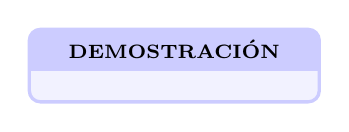
\begin{tikzpicture}
	\node [demoBox](box){%
		\textbf{\scriptsize 
			DEMOSTRACIÓN}
		\nodepart{two}
		\begin{minipage}{\textwidth}
		\vspace*{0.1cm}
		\BODY
		\end{minipage}
	};
	\end{tikzpicture}
\end{center}
}

\NewEnviron{demoPart}[1][]{%
	\begin{center}
		
\begin{tikzpicture}
		\node [demoPart](box){%
			\begin{minipage}{0.75\textwidth}
			\vspace*{0.1cm}
			\BODY
			\end{minipage}
		};
		\end{tikzpicture}
	\end{center}
}

\newcommand*{\theadc}[1]{\multicolumn{1}{|c|}{\bfseries #1}}
\newcommand*{\thead}[1]{\multicolumn{1}{c}{\bfseries #1}}
\newcolumntype{Y}{>{\centering\arraybackslash}X}


